\subsection{Working with models in \jb{}}
\protect\gdhelpid{org.eclipse.ui.resource_view_context}{Navigator View}
\index{Modeling}

The \app{} modeling perspective has been designed to help teams get started with automated testing early on in the development process by allowing the import of UML diagrams and the subsequent generation of \gdcase{} structures from the models. 

Testing early is important to find errors when they are cheaper to fix, yet it is often difficult to know where to start testing or how to structure the tests to be as reusable and maintanable as possible. 

At this stage, it is important to realize that the aim is not to derive complete, functional tests from complex models. Instead, the imported use case diagrams and activity diagrams, and the \gdcases{} generated from them, can be used to see which structures (\gdcases{}) will need to be reused throughout the test, and what sequences of \gdcases{} will need to be created to cover the use cases. 





\subsection{Creating a \gdproject{} for modeling}
\protect\gdhelpid{org.eclipse.ui.resource_view_context}{Navigator View}
\label{TasksMBTCreateProject}
\index{Project!Create for Model}
\index{Create Model Project}

The first thing to do when you want to work with models in \app{} is to create an Eclipse Project in which the models will be managed and saved. The \gdproject{} will be saved in your workspace. 

\begin{enumerate}
\item Switch to the modeling perspective if you have not already done so. You can do this by selecting:\\
\bxmenu{Window}{Open Perspective}{Modeling Perspective}
\item In the \gdnavview{}, click the \bxcaption{Create New Project} button
or select:\\
\bxmenu{New}{Project}{}\\
from the context-sensitive menu. 
\item In the wizard that appears, select \bxname{Project} from the \bxname{General} category. 
\item Click \bxcaption{Next}
\item Enter a \gdproject{} name. You can decide whether to keep the \gdproject{} in your workspace or link to it from your workspace. 
\item Click \bxcaption{Finish}. The \gdproject{} you just created will appear in the \gdnavview{}. It contains the file \bxname{.project}. Do not delete this file!
\item Now you have created a \gdproject{}, you can create a new model diagram \bxpref{TasksMBTCreateModel} or import models \bxpref{TasksMBTImport}. 
\end{enumerate}


\subsection{Creating a new model diagram}
\protect\gdhelpid{org.eclipse.ui.resource_view_context}{Navigator View}
\gdhelpid{newModelWizardContextId}{New Model Wizard}
\label{TasksMBTCreateModel}
\index{Modeling!Create Model Diagram}
\index{Model Diagram!Create}


To be able to create a model, you must first have created a \gdproject{} in the \gdnavview{} \bxpref{TasksMBTCreateProject}. 

\begin{enumerate}
\item In the \gdnavview{}, click the \bxcaption{Create New \gdcase{} Model} button select:\\
\bxmenu{New}{Other}{}\\
from the context-sensitive menu. 
\item In the wizard that appears, select \bxname{Test Case Model} from the \bxname{Models} category. 
\item Click \bxcaption{Next}. 
\item Select or enter the \gdproject{} you want to create the diagram in. 
\item Name the new model. 
\item Click \bxcaption{Finish}. The model diagram you created will appear in the \gdnavview{} in the \gdproject{} you specified. The \gdmodeleditor{} will open. \item Now you have created a model diagram, you can add elements to it to model your test \bxpref{TasksMBTModel}. 
\end{enumerate}


\subsection{Importing models from UML}
\protect\gdhelpid{org.eclipse.ui.resource_view_context}{Navigator View}
\gdhelpid{importModelWizardContextId}{Import Model Wizard}
\label{TasksMBTImport}
You can export and import your \gddb{} preferences for \app{}. This makes migrating to new versions easier, as you do not have to reenter any \gddb{} preferences. 

To export your \gddb{} preferences:
\begin{enumerate}
\item Select: \\
\bxmenu{File}{Export}{}\\
from the main menu in the \ite{}. 
\item In the dialog that appears, select: \bxname{General/Preferences} and click \bxcaption{Next}.
\item Select the \bxname{Database Connections} option and browse to a place in the file system where you want the preferences to be saved. 
\item Click \bxcaption{Finish}.
\end{enumerate}

To import your \gddb{} preferences:
\begin{enumerate}
\item Select: \\
\bxmenu{File}{Import}{}\\
from the main menu in the \ite{}. 
\item In the dialog that appears, select: \bxname{General/Preferences} and click \bxcaption{Next}.
\item Browse to the preference file you wish to import. 
\item Select the \bxname{Database Connections} option and click \bxcaption{Finish}.
\end{enumerate}



\subsection{Creating models: adding \gdcases{}, categories, parameters and referenced \gdcases{}}
\gdhelpid{guidancerModelEditorContextId}{Modeling Editor}
\label{TasksMBTModel}
\index{Event Handler!Add}
\index{Add!Event Handler}



This section deals with adding \gdehandlers{} to \gdcases{}.  For information on using \gdehandlers{} meaningfully to ensure that your test execution is as robust as possible, see the section on \gdehandlers{} in the Best Practices section \bxpref{BPEHandlers}. 

\begin{enumerate}
\item Open the \gdtestcaseeditor{} by double-clicking on the \gdcase{} you want to edit in the \gdtestcasebrowser{}.   
\item Select\\
\bxmenu{Add}{\gdcase{} as \gdehandler{}}{} \\from the context-sensitive menu in the editor or use \bxkey{Ctrl+Enter}. 

\bxtipp{You can also drag the \gdcase{} you want to use straight into the \gdehandlers{} area of at the bottom of th the \gdtestcaseeditor{}. }

\item Choose a \gdcase{} to add from the dialog that appears.
\bxtipp{You can't add a \gdcase{} to itself as an \gdehandler{}, because this would create an infinite loop. }
\item Select an event type from the combo box \bxpref{eventtype}.
\item Select a reentry type from the combo box \bxpref{reentrytype}. 
\bxtipp{For each \gdcase{} you can only add one \gdehandler{} for each event type.}
\item Click \bxcaption{OK}. 
\item The \gdehandler{} appears in the lower half of the \gdtestcaseeditor{}. 
\gdmarpar{../../../share/PS/EventHandler}{ \gdehandler{}}
\item Save the changes in the editor.
\end{enumerate}




\subsection{Altering the appearance of models}
\gdhelpid{guidancerModelEditorContextId}{Modeling Editor}
\index{Modeling!Appearance}
\index{Appearance!Model}

There are various ways of altering the appearance of the model and the canvas. 

In the main menu, under the \bxname{Modeling} menu, you can alter details about the fonts, colors and lines as well as choosing whether to show grids and rulers. These options are also available in the \gdpropview{} in the modeling perspective under the \bxname{Appearance} and \bxname{Rulers \& Grid} tabs. 

You can also set appearance features in the preferences for modeling \bxpref{TasksPrefsModel}. 



\subsection{Options for working with models: zoom, print, undo etc.}
\gdhelpid{guidancerModelEditorContextId}{Modeling Editor}
\index{Modeling!Options}


The modeling perspective offers different ways of grouping and visualising your model, as well as useful actions to help you work with the model:

\begin{description}
\item [Zooming:]{You can use the context-sensitive menu and the main menu to zoom into and out of the canvas. }
\item [Printing:]{In the context-sensitive menu for the canvas, you can opt to print the model. In the main menu you can choose to see page breaks in the \gdmodeleditor{}. }
\item [Saving as an image:]{You can save the model as an image file using the context-sensitive menu in the \gdmodeleditor{}. }
\item [Undo, Redo, Cut, Copy and Paste]{ actions are all available in the context-sensitive menu in the \gdmodeleditor{}. }
\item [Arranging:]{You can either arrange the selected items in the \gdmodeleditor{} or arrange all of the items automatically.}
\item [Adding notes:]{You can add notes to the model and to the elements within it. Notes are, however, not generated with the \gdcases{} from the model.}
\end{description}




\subsection{Generating \gdcases{} and categories from models}
\gdhelpid{generationWizardContextId}{Generating Models}
\gdhelpid{guidancerModelEditorContextId}{Modeling Editor}
\label{TasksMBTGenerate}
\index{Generate Model}
\index{Modeling!Generate}

In order to be able to generate \gdcases{} and categories from a model, you must have:
\begin{itemize}
\item Created a modeling \gdproject{} \bxpref{TasksMBTCreateProject}.
\item Created \bxpref{TasksMBTCreateModel} or imported \bxpref{TasksMBTImport} a model diagram.
\item Created \bxpref{newproject} or opened \bxpref{loadproject} a \gd{} \gdproject{}. 
\end{itemize}

\begin{enumerate}
\item When you are ready to generate, select:\\
\bxmenu{Modeling}{Generate}{}\\ from the menu or select the \bxcaption{Generate} button on the toolbar \gdmarpar{../../../share/PS/transform}{Generate}.
\item In the dialog that appears (\bxfigref{GenerateDialog}), you can configure what you want to generate. 

\begin{figure}[h]
\begin{center}
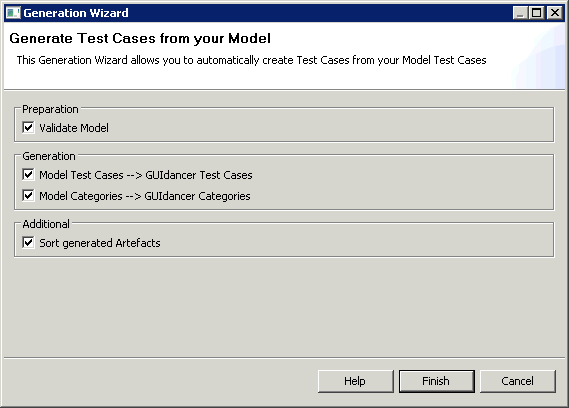
\includegraphics{Tasks/Modelling/PS/GenerateDialog}
\caption{Generation Dialog}
\label{GenerateDialog}
\end{center}
\end{figure} 


\begin{description}
\item [Validating]{ the model is the prerequisite for all other options. It ensures that the model can be successfully generated.} 
\item [Model \gdcases{} to \gd{} \gdcases{}:]{This converts any \gdcases{} you have created in the model to corresponding \gd{} \gdcases{} in the \gdtestcasebrowser{}. Generated \gdcases{} have a green corner. }
\item [Model categories to \gd{} categories:]{This converts categories you have created in the model to categories in the \gdtestcasebrowser{}. Generated categories are slightly green. }
\item [Sort generated artefacts:]{This option organizes your \gdcases{} into categories as specified in the model. If you turn this option off, your \gdcases{} will not be created in the modeled categories, nor will any \gdcases{} from previous generations be moved back into the modeled categories in the \gdtestcasebrowser{} (if you re-organized \gdcases{} for example).}
\end{description}
\item Click \bxcaption{Finish} to start the generation. During the generation, the status of the various actions is shown in the console. Once the generation is complete, you will be able to see the items you generated in the \gdtestcasebrowser{}. 
\bxtipp{Parameters that are part of generated \gdcases{} are \bxname{locked} by default, and cannot be changed or deleted. You can see the parameters and unlock them in the \gdtestcaseeditor{} using the \bxname{edit parameters} dialog \bxpref{editparams}. }
\item Once the \gdcases{} have been generated, you can fill them with the necessary \gdcases{} from the library in \gd{} to create your tests. 
%regeneration, model always right
\end{enumerate}

\subsubsection{Regenerating models}
After generating a model for the first time, you may want to make changes and regenerate it. This is not a problem in \gd{} -- it will not result in duplicates of previously created items being made. Any changes made to the model (if you have added or renamed items, for example) will be reflected in the \gdcase{} generation. However, there are two points to bear in mind:

\begin{description}
\item [Deleting objects from the model:]{Any objects you delete from the model will not be deleted from the \gdcase{} browser. }
\item [The model takes precedence over other changes:]{If you have made changes to the generated \gdcases{} in the \gdtestcasebrowser{} or \gdtestcaseeditor{} (e.g. renamed them, added other \gdcases{}), these changes will be lost when you regenerate the model. }
\end{description}


\subsection{Validating models}
\gdhelpid{guidancerModelEditorContextId}{Modeling Editor}
\label{TasksMBTValidate}
\index{Validate Model}
\index{Modeling!Validate}

You can validate your model at any time by selecting:\\
\bxmenu{Modeling}{Validate}{}. \\


Or by clicking the \bxcaption{validate} button on the toolbar.
The validation ensures that the model is fit to be generated, and does not contain any errors. 
\gdmarpar{../../../share/PS/validate}{Validate}

If there are errors in the model, you will see this in the console output. In the \gdmodeleditor{} itself, the places with errors will be marked with a red cross. Hovering over the cross will show a tooltip with information on the error (\bxfigref{ModelError}). 

\begin{figure}
\begin{center}
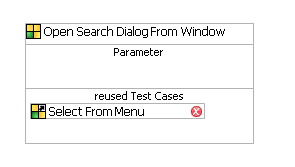
\includegraphics{Tasks/Modelling/PS/ModelError}
\caption{Model showing an error}
\label{ModelError}
\end{center}
\end{figure} 


%in UI stuff - the modeling perspective
